\scanpage{20}
\deleted{\unsure{symétrique} \unsure{additif}}
\figure{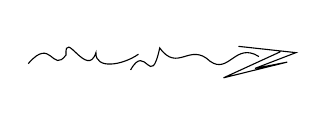
\begin{tikzpicture}[x=1cm,y=1cm]
\draw (0,0) .. controls (.3,.35) and (.3,-.13) .. (.48,.11)
 .. controls (.46,.45) and (.75,-.2) .. (.86,.14)
 .. controls (.85,-.08) and (1.2,-.02) .. (1.4,.12);
\draw (1.3,-.08) .. controls (1.5,.28) and (1.55,-.35) .. (1.67,.2)
 .. controls (1.9,-.12) and (2.05,.28) .. (2.31,.03)
 .. controls (2.55,-.14) and (2.63,.28) .. (2.93,.09);
\draw (2.67,.22)--(3.40,.14)--(2.88,-.06)--(3.29,.02)--(2.48,-.18)--(3.20,.15);
\end{tikzpicture}}
\[
 \begin{aligned}
 X^p+A_1(X_1,-,X_n)X^{p^{n-2}}+A_2(X_{\unsure{2|1}},-\,X_n)X^{p^{n-3}}\ \text{---}\\
 {}+A_{n-1}(X_1,-X_n)X
 \end{aligned}
\]

% margin note written sideways
\margin{\scriptsize
$H_0\quad G_0\quad K_0=G_0/H_0$

$G/\bar H_0=\bar G_0/\bar H_0=\bar K_0$

$G/H=K$
\diagram{\resizebox{\marginparwidth}{!}{\begin{tikzcd}[ampersand replacement=\&,column sep=small,row sep=small]
G_0\arrow[r]\&K_0\arrow[r,"\unsure{=|\sim|\Rightarrow}"]\&K_0\\
G\arrow[r,"{\deleted{\unsure{K}}}"]\&\bar K_0\arrow[r,"?"]\&\bar K\\
\&G/H\arrow[u,equal]\&
\end{tikzcd}}}
\diagram{\resizebox{\marginparwidth}{!}{\begin{tikzcd}[ampersand replacement=\&,row sep=tiny,column sep=small]
{}\arrow[r,dash]\&H_0\arrow[r,dash]\&G_0\arrow[r,dash]\&K_0^{\unsure{r|0}}\arrow[r]\&0\\
\&\&\&\unsure{\varepsilon|\xi}\arrow[u,"{\unsure{f}}"]\&\\
\&\&\&K_0\arrow[u]\&\\
\&\&\&\bullet\arrow[u,dash]\&
\end{tikzcd}}}
$\underbrace{\hphantom{G_0\quad K_0\quad0}}$

$\operatorname{Hom}(\alpha_{p^r},G_a)$

$\shortparallel$

$\operatorname{Hom}(\alpha_{p^r},\alpha_{p^r})$

$V=0,\ F^r=0\quad p=\unsure{0|\bullet}$

$\mathbb F_p(\unsure{F|E|\mathbb F})/F^r$}

\[
 \begin{aligned}
 X_1\check e_1+\text{---}+X_n\check e_n\\
 X_1^p\check e_1\qquad X_n^p\check e_n\\
 X_1^{p^{n-1}}\check e_1\qquad X_n^{p^{n-1}}\check e_n
 \qquad&\lambda^{1+p+\text{---}\,p}\\
 X_1^{p^n}\check e_1\qquad X_n^{p^n}\check e_n
 \qquad&\lambda^{p^n-p^{n-1}}\quad\lambda^{p^n-p^{n-2}}
 \end{aligned}
\]
\[
 X_1^{p^n}+a_1X_1^{p^{n-1}}+a_2X_1^{p^{\unsure{n-1|n-2}}}\ \text{---}
 +a_nX_1=0
\]
\figure{
\begin{tikzpicture}[x=1cm,y=1cm]
\draw (0,.25) .. controls (.06,-.25) and (.31,-.11) .. (.21,.17)
 .. controls (.20,.35) and (.14,-.16) .. (.41,-.04);
\foreach \x in {.40,.55,.70,.85,1.0}
 {\draw (\x,-.04) .. controls (\x+.21,.00) and (\x+.03,.34) .. (\x+.01,.16)
 .. controls (\x-.04,-.04) and (\x+.08,-.13) .. (\x+.17,-.02);}
\draw (1.15,-.02)..controls(1.35,.02)and(1.32,-.13)..(1.49,.02);
\end{tikzpicture}}
\[
 {f}^{p^{\unsure{n}}}+a_1 f^{p^{n-1}}\ \text{---}
 +a_{n-1}f^{\unsure{p}}+a_n f=0
\]
\figure{\begin{tikzpicture}[x=.55cm,y=.55cm]
\draw (0,0)..controls(.50,.12)and(.04,.72)..(.34,.69)
 ..controls(.82,.63)and(.17,1.28)..(.56,1.12)--(.91,.95);
\end{tikzpicture}}
\[
 \begin{aligned}
 f&\quad f^p\quad\text{---}\quad f^{p^{n-1}}\\
 e_1&\quad e_2\hspace{4.2em}e_n
 \end{aligned}
\]
\[
 \begin{aligned}
 e_1^{(p)}&\longmapsto e_2\\
 e_2^{(\unsure{p|n})}&\longmapsto e_3\\[-3pt]
 &\cdots\\
 e_{n-1}^{(p)}&\longmapsto e_n\\
 e_n^{(p)}&\mathrel{\unsure{\rule{1.3em}{.4pt}|\mapsto}}a_1 e_n+a_2 e_{n-1}\ \text{---}+a_{\text{\uuline{$n$}}}e_1\\
 &a_n\ne0
 \end{aligned}
\]
\figure{\begin{tikzpicture}[x=.55cm,y=.55cm]
\draw (0,0)..controls(.40,.04)and(.0,.65)..(.37,1.03)
 ..controls(.72,1.5)and(.20,1.95)..(.64,1.90)
 ..controls(1.13,1.78)and(.55,2.39)..(.93,2.27)
 ..controls(1.26,2.15)and(.70,2.57)..(1.13,2.45);
\end{tikzpicture}}
\[
 \begin{aligned}
 e_1^p=e_2\quad e_2^p=e_3\ \text{---}\quad e_{n-1}^{p}=e_n,\quad
 e_n^p={}&-(\unsure{a_1}e_n+a_2e_{n-1}\\
 &{}+a_ne_1)
 \end{aligned}
\]
\[
 \begin{aligned}
 \underset{\text{loc. \unsure{li.|l.|lib.} t.f.}}M\qquad&M^{(p)}\xrightarrow{\sim}M
   \qquad\underline M\longrightarrow\underline O\\
 &e_1\ \text{--}\ e_n\qquad e_i^p\mathrel{\unsure{\rule{1.3em}{.4pt}|\to|\mapsto}}\sum_j\lambda_{ij}e_j
 \end{aligned}
\]
\[
 M\to M^{(p)}\longrightarrow\underline M\qquad \unsure{x^p|xp}
\]
% archive sheet number: 19
